\chapter{Optimizations}
\label{chap:5}

Upon publishing, $\plonk$ became a popular SNARK, and variants of the protocol have been implemented in many cryptocurrency projects. This led to efforts to make the protocol more efficient. The optimizations can be done on three fronts:
\begin{itemize}
    \item Polynomial commitment scheme 
    \item Interactive Protocol
    \item Recursive proof composition
\end{itemize}

\section{Possibilities for optimization}
\label{optimization-possibilities}

\subsection{Polynomial commitment scheme:} The $\plonk$ protocol was initially described with the KZG \cite{KZG} polynomial commitment scheme, but other polynomial commitment schemes like FRI \cite{fri} could be used as well. As mentioned, commitments realized by MSM place a large computational load on the prover. One of the authors of $\plonk$ has already written a follow-up article on the construction of efficient polynomial commitment schemes for multiple points and polynomials \cite{shplonk} that can be used in $\plonk$.

\subsection{Interactive protocol:} This covers the rest of the protocol that is not about the polynomial commitment scheme. The possibilities for optimization range from more effective arithmetization to constructing more efficient polynomial checks. The major work in this area was done on the use of custom gates and the construction of lookup tables. By using more complex custom gates, it is possible to reduce the degree of the circuit, which determines the complexity of the prover. Custom gates are described in detail in \textit{TurboPlonK} \cite{turboplonk}. The lookup tables from \textit{plookup} \cite{plookup} enable to precompute values for inputs $\publicinput$ and then prove that the witness $\witness$ exists in that table. These two approaches are independent and can be combined, as shown in \textit{HyperPlonK} \cite{HyperPlonk}.

\subsection{Recursive proof construction:} SNARKs place most of the computational load on the prover. Since the verifier is considered to be computationally weak, the verification algorithm is designed to lightweight and effective. Nevertheless, optimizing the verifier for multiple proofs is possible. The technique of recursive proof composition can aggregate several proofs into a single one and provide proof that each of the sub-proofs is valid. This approach is formalized in the  \textit{Halo} protocol \cite{halo}, where the authors introduced an accumulation layer of the proof system.

\section{ZK-Garage PlonK}
In this work, I  use \href{https://github.com/ZK-Garage/plonk}{ZK-Garage} as a reference implementation of $\plonk$. ZK-Garage is an open-source Rust implementation that uses arkworks library \cite{arkworks} for cryptographic primitives, arithmetic operations, and other utilities. The implementation adds the mentioned lookup tables and extends the arithmetic gates with AND, XOR, and range gates.

\begin{figure}
    \centering
    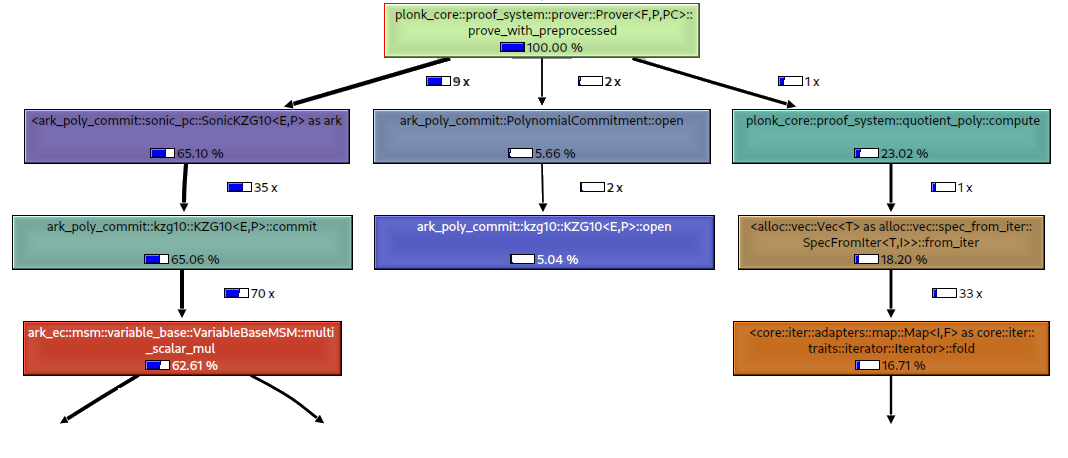
\includegraphics[width=1\linewidth]{figures//optimizations/computation_load.png}
    \caption{Computational Load of ZK-Garage implementation}
    \label{fig:profiler}
\end{figure}

Before trying out possible improvements, I analyzed demanding parts of the code. I used the popular profiling tool \textit{Callgrind} for that task. It monitors how often each function is called, along with the number of CPU instructions executed within each function. This allows for identifying the most computationally demanding function and prioritizing the efforts to ensure that the optimizations have the most significant impact on overall performance. 

The prover algorithm is contained in the function \texttt{prove\_with\_preprocessed}, which takes common preprocessed input as an argument. Figure \Cref{fig:profiler} shows the most demanding computation of the prover in a call graph. The most computationally heavy parts of the program are the computation of commitments and the construction of the quotient polynomial $t(x)$. From the computation of the prover algorithm, 65\% of the CPU instructions were spent on the commitments to the polynomials and 23\% on the construction of the quotient polynomial. The function that calculates the quotient polynomial is called only once, and there are two calls to polynomial openings at $\mathfrak{z}, \mathfrak{z}\omega$. As specified in the protocol, nine polynomial commitments correspond to the calls of the \texttt{commit} function. The profiler was executed on  $\textit{BenchCircuit}$ of size $2^{6}$, and the relative computation load varied depending on the circuit size. Nevertheless, most of the time is spent calculating commitments and the quotient polynomial $t(x)$, so optimizing it will be the goal for the rest of this chapter. Minimizing the number of commitments would mean the checks could be encoded more efficiently with fewer polynomial. This task is complex, but there are other ways to improve the performance. For example, it is possible to reduce the size of MSM in some of the commitments.

\section{Wire polynomials degree reduction}
In this work, I aimed to give a detailed explanation of the prover algorithm in the interactive protocol and decided to think of possible improvements in this area. I led a discussion on potential improvements with Tomáš Krňák \cite{tomas}, who suggested looking at the construction of wire polynomials $a(x), b(x), c(x)$, which are interpolated from the witness $\witness$. 

ZK-Garage interpolates $a(x), b(x), c(x)$ using inverse Fast Fourier transform ($\ifft$) implemented in \textit{arkworks}. The library calculates $\ifft$ using a variant of the Cooley–Tukey algorithm \cite{cooley-fft}, which requires the number of evaluations to be a power of two. The wire polynomial computed in round 1 also determines the degree of the polynomials computed in the following rounds. Reducing the degree of $ an (x), b(x), c(x)$ naturally speeds up the computation of $[a]_1, [b]_1, [c]_1$, but the construction and commitment of the quotient polynomial should also be faster. This makes it a meaningful candidate for optimization.

I have tried to reduce the degree of $a(x), b(x), c(x)$ in two ways suggested by Tomáš Krňák. It is possible to perform the reduction by polynomial division in coefficient form and also by pairwise division in evaluation form. The two approaches are sketched in the diagram \Cref{fig:degree-reduction}.

\subsection{Problem statement} 
The problem with the current implementation is that wire polynomials may be at most twice as big as the size of the circuit because of the padding to the next power of two. We denote the wire vector as $w = \{w_0, w_1 \ldots w_{m-1}\}$. The closest power of two to $m$ is $n$. To interpolate $w$ using $\ifft$, it needs to be padded to size $n$, which means that the size of SRS needs to be at least $n$. In the ZK-Garage, $w$ is padded with $n-m$ zeros. We denote the interpolated polynomial as: $$W(x) = w(x)pad_0(x)$$,
where $w(x)$ is defined by $w$ on the evaluation domain $H = \{1, \omega, \ldots \omega^{m-1}\}$ and $pad_0(x)$ is polynomial which has roots on $\{\omega^m, \omega^{m+1}, \omega^{n-1}\}$. We can write the padding polynomial as: 

\begin{equation}
    \label{padding-polynomail}
    pad_0(x) = (x - \omega^m)(x - \omega^m+1) \ldots (x - \omega^{n-1})
\end{equation}.

The reference implementation wire vector is padded and interpolated. There is no further degree reduction which means that $a(x), b(x), c(x)$ have degree $n-1$. It is also worth noting that the protocol does not perform any checks on the padding domain  $[\omega^{m}, \omega^{n-1}]$, which means we can pad the vectors with arbitrary values. As shown in the \Cref{chap:2}, the prover needs to show the following checks hold:

\begin{enumerate}
    \item Public input check: the public input is encoded in the first $l$ indices of the witness $\witness$, so values on $[\omega^{m}, \omega^{n-1}]$ do not concern it.
    \item Output check: the circuit output check verifies evaluation of the last element in the witness on $\omega^{m-1}$, therefore $[\omega^{m}, \omega^{n-1}]$ are not relevant for this case.
    \item Gate check: the values of the selectors $q_m(x), q_l(x), q_r(x), q_o(x), q_(x)$ on $[\omega^{m}, \omega^{n-1}]$ are zero because they do not encode any gate. Since $a(x), b(c), c(x)$ in the gate equation \Cref{gate-constraint} are always in combination with some selector the whole expression will evaluate to 0 as it should.
    \item Wiring check: the permutation function the the range $[\omega^{m}, \omega^{n-1}]$ encodes identity. This means that the wiring check does not enforce anything on $[\omega^{m}, \omega^{n-1}]$.
\end{enumerate}

Next, we present two optimizations that aim to use $\ifft$ to get $W(x)$ and reduce its degree to get $w(x)$. In the following sections, each approach will be described in detail.

\begin{figure}[H]
    \centering
    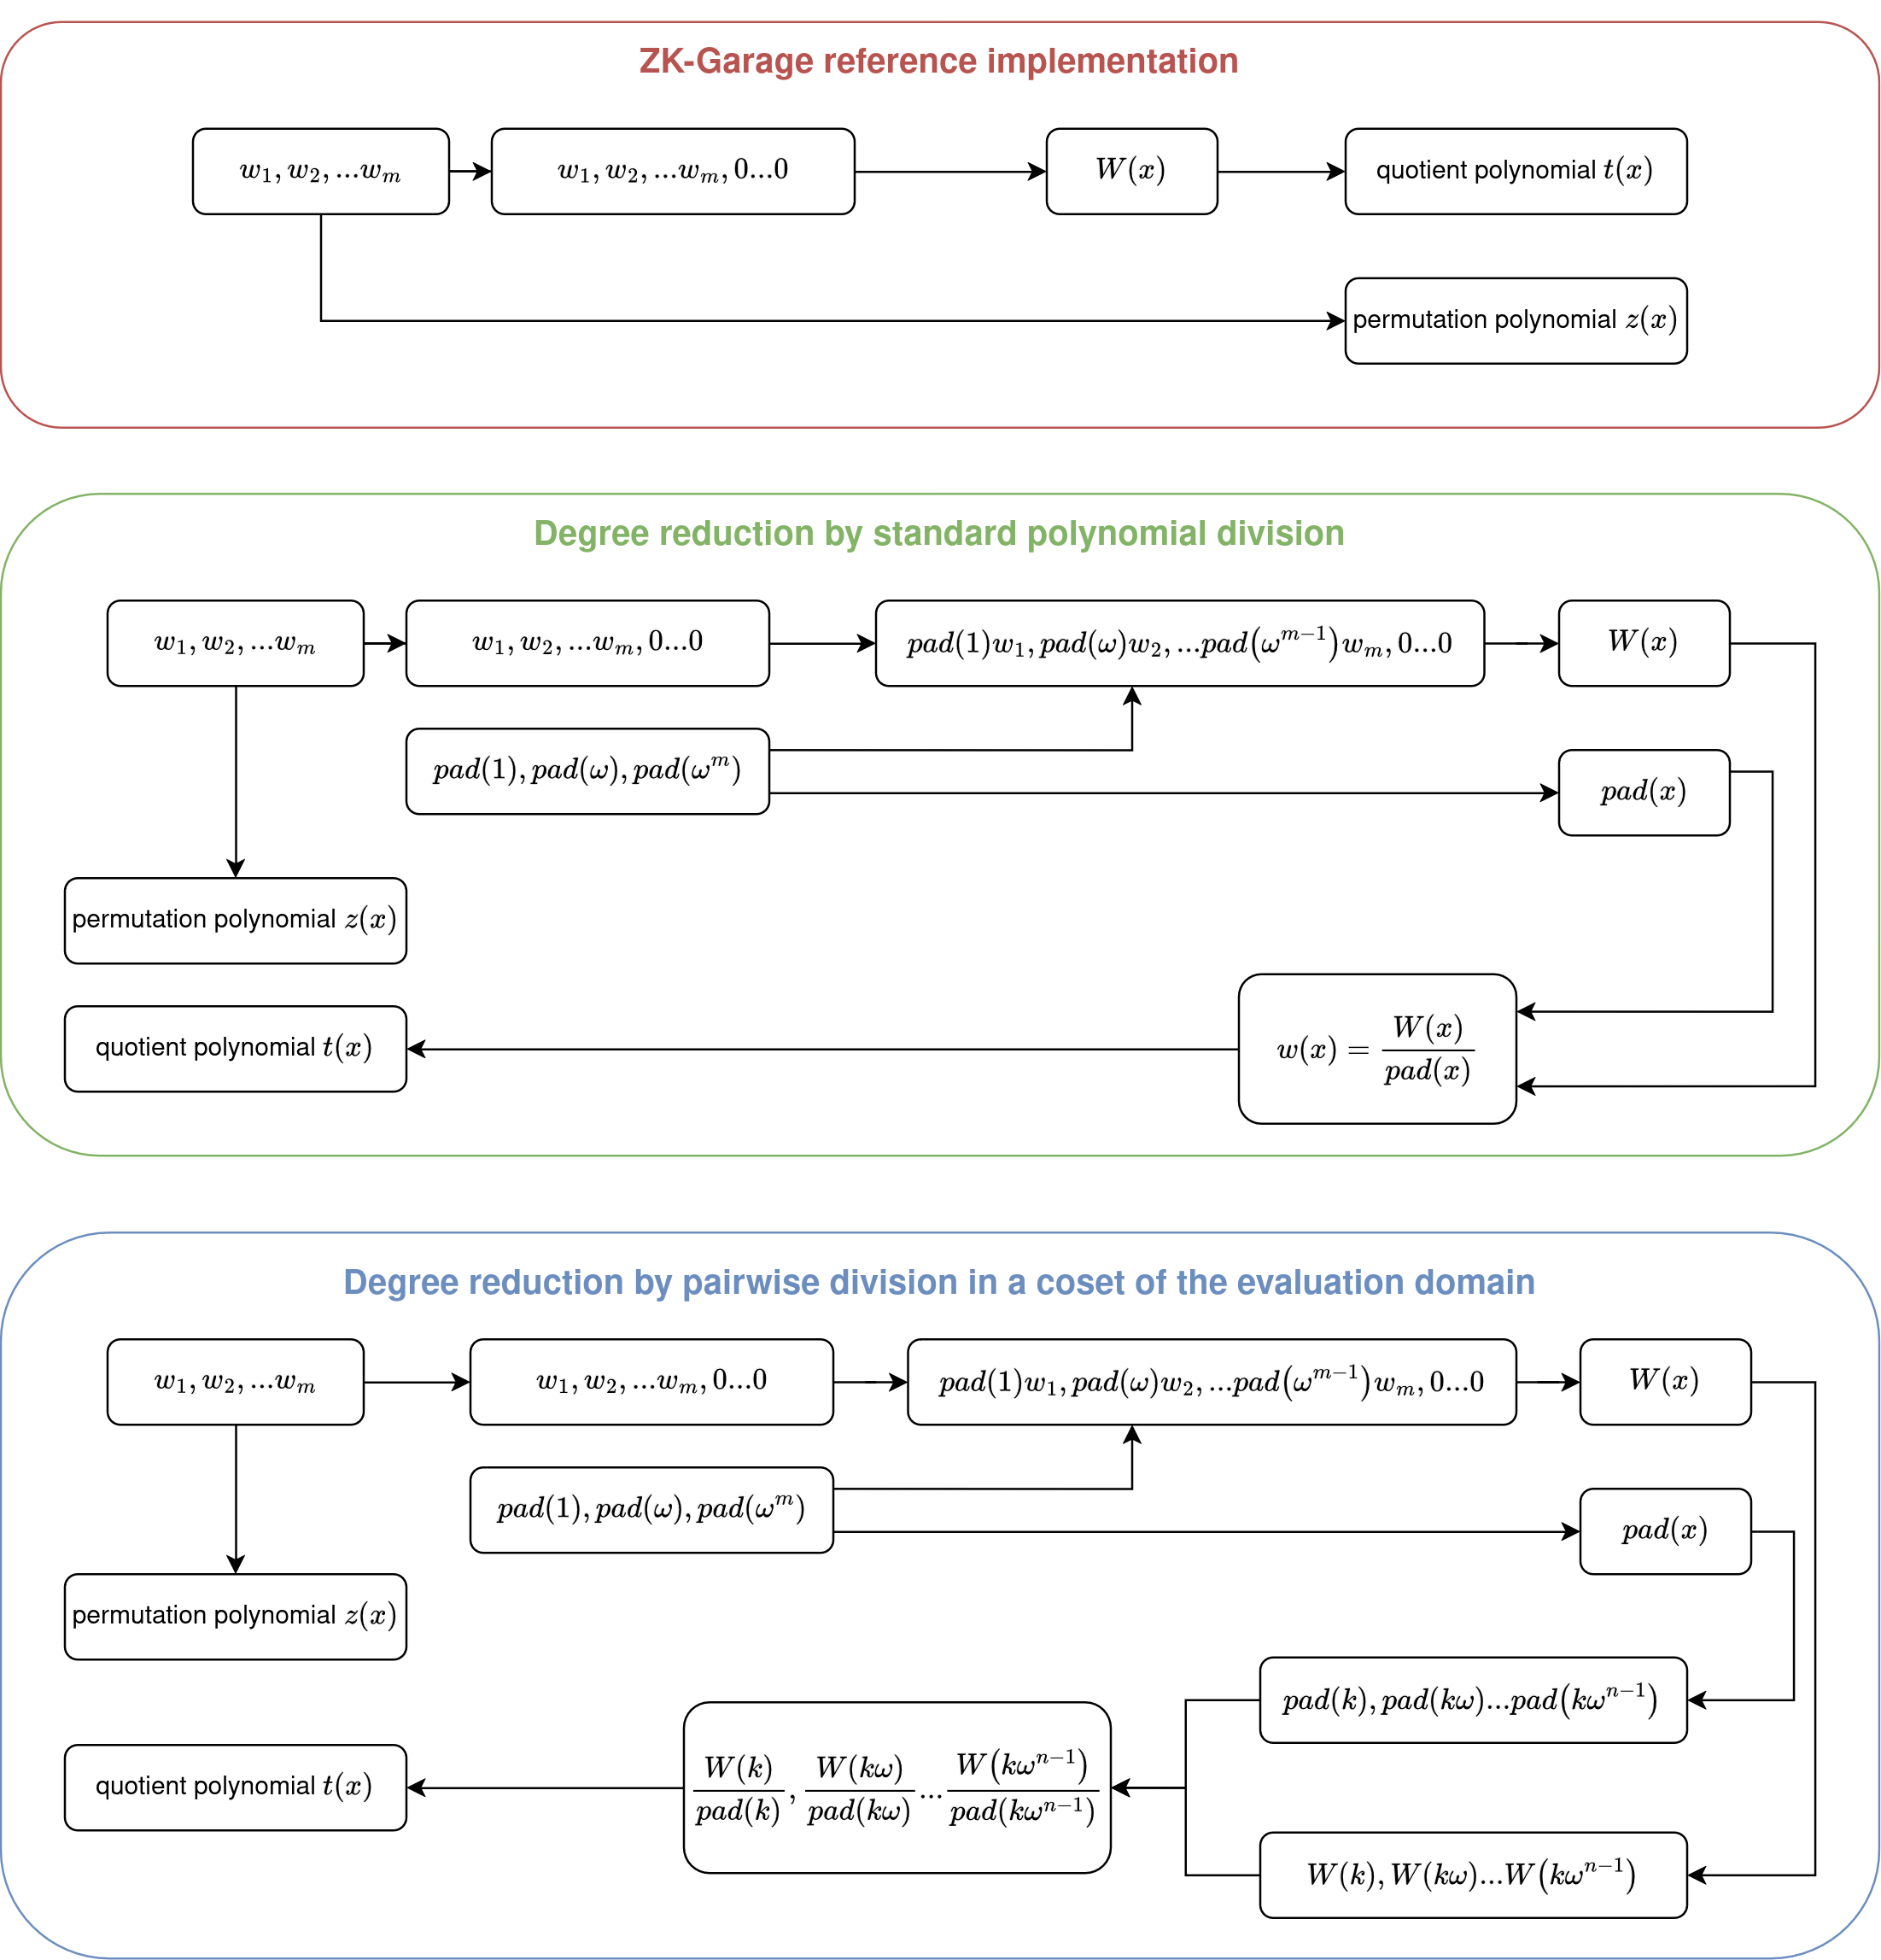
\includegraphics[width=1\linewidth]{figures/optimizations/degree_reduction_diagram.drawio.png}
    \caption{Degree reduction variants}
    \label{fig:degree-reduction}
\end{figure}

\subsection{ZK-Garage implementation}

\begin{pchstack}[center, boxed]
    \pseudocode[linenumbering, head=\textcolor{red}{Reference implementation in ZK-Garage}] {
        \text{construct padding vector } [0]^{n-m} \\
        \text{concatenate } [w, [0]^{n-m}] \\
        \text{interpolate } W(x) = \ifft(w, [0]^{n-m}) \\
        \pcreturn W(x)
    }
\end{pchstack}

The prover algorithm receives wire vectors $w_l, w_r, w_o$. These are padded with zeros and interpolated by $\ifft$ over the domain $H$ to get polynomial $a(x), b(x), c(x)$. Padded wire vectors are further used to calculate the permutation polynomial in \hyperref[chap:round2]{round 2} because, according to the protocol, the permutation polynomial is computed in the evaluation form.

\paragraph{Time analysis:} The complexity of this approach is dominated by $\ifft$, which has complexity $\bigO{n \log{n}}$.

\definecolor{ultramarine}{rgb}{0, 0.501, 0}
\subsection{Polynomial division}
\begin{pchstack}[center, boxed]
    \label{poly-div}
    \pseudocode[linenumbering, head=\textcolor{ultramarine}{Reduction by polynomial division}] {
        \text{construct padding vector } [0]^{n-m} \\
        \text{evaluate } [pad_0(1), pad_0(\omega), \ldots, pad_0(\omega^{m-1})] \\
        \text{concatenate } [w, [0]^{n-m}] \\
        \text{pair-wise multiplication } \Tilde{w} = [w_0 pad_0(1), \ldots w_{m-1} pad_0(\omega^{m-1}), 0 \ldots 0] \\
        \text{interpolate } W(x) = \ifft(\Tilde{w}) \\
        \text{reduce degree by polynomial division } w(x) = W(x) / pad_0(x) \\
        \pcreturn w(x)
    }
\end{pchstack}

The most straightforward approach when reducing the degree is to perform polynomial division by the polynomial defined by the padding values on $\{\omega^m, \ldots, \omega^{n-m}\}$. Note that $[w_0, w_1 \ldots w_{m}]$ first needs to be pair-wise multiplied by $[pad_0 \ldots pad_{m}]$ so that it holds $W(x) = w(x)pad(x)$. In this approach, I have used the standard algorithm for long polynomial division. As a result, it is possible to retrieve $w(x)$ of degree $m$ and use it in the following approach. The padded vector $[w_1, \ldots w_{m-1}, 0 \ldots 0]$ is again used in the round 2 to calculate $z(x)$. 

The zero padding polynomial could be written as $pad_0(x) = \prod_{i=m}^{n-1} (x - \omega^i)$. Computing values $[pad_0(1), pad_0(\omega) \ldots pad_0(\omega^{m-1})]$ requires significant number of field operations. There are $n-m$ field multiplications needed to calculate value $pad(\omega^i)$. To compute values on $[1 \ldots \omega^{m-1}]$, it is needed to perform $n-m \times m = nm - m^2$ field multiplication, which introduces non-negligible overhead. Luckily there is a better approach and evaluation of $pad_0(x)$ on $[1, \ldots \omega^m]$ can be calculated using recursive formula:
\begin{equation}
    \label{eq:recursive-formula}
    pad_0(x) =
    \begin{cases}
        \prod_{j=m}^{n-1} (1 - \omega^j) & x = 1,  \\
        \omega^{n-m-1} \frac{\omega^{i-1} - \omega^{m-1}}{\omega^{i-1} - \omega^{n-1}} pad_0(\omega^{i-1}) & x = \omega^i: i \in [m] \setminus \{1\}
    \end{cases}
\end{equation}

To confirm the correctness of this formula:
$$\frac{pad_0(\omega^i)}{pad_0(\omega^{i-1})} = \prod_{j = m}^{n-1} \frac{\omega^i - \omega^j}{\omega^{i-1} - \omega^j} = \omega^{n-m} \prod_{j = m}^{n-1} \frac{\omega^{i-1} - \omega^{j-1}}{\omega^{i-1} - \omega^j}$$
$$= \omega^{n-m} \frac{\omega(\omega^{i-1} - \omega^{m-1})}{\omega^{i-1} - \omega^{n-1}} = \omega^{n-m} \frac{\omega(\omega^{i-1} - \omega^{m-1})}{\omega^{i-1} - \omega^{n-1}}$$
$$pad_0(\omega^i) = \omega^{n-m} \frac{\omega(\omega^{i-1} - \omega^{m-1})}{\omega^{i-1} - \omega^{n-1}}pad_0(\omega^{i-1})$$


\paragraph{Time analysis:} Calculating evaluations of $pad$ can be done in $m$ iteration thanks to the recursive formula \Cref{eq:recursive-formula} and pairwise multiplication in step 4 of the algorithm could be trivially parallelized. Naive polynomial division, which has  complexity $deg(w(x))\times deg(pad_0(x)) = n \times n-m$, which makes the total complexity $n^2 - nm + n\log{n}$. Since $m < n/2$  we can conclude $\bigO{n^2 - \frac{3}{2}n}$.

From the analysis, we can already conclude that this approach will be much slower in round 1 than the former implementation. However it is questionable what is the performance benefit in rounds 2 - 5. As suggested by Tomáš Krňák \cite{tomas}, padding the circuit with a sparse polynomial might slightly speed up the polynomial division. One possibility is to use padding polynomial $pad_{cyclic}(x)$ that is zero on every $k$-th element of $H$ instead of  $pad_0(x)$ which is zero on $[\omega^m \ldots \omega^{n-1}]$, i.e.,

\begin{equation}
    pad_{cyclic}(x) = x^{\frac{n}{k}} - 1
\end{equation}.

The domain $H$ is generated by the $n$-th root of unity, so for every $\omega^ki$ it holds that:

$$pad_{cyclic}(\omega^{ki}) = \omega^{ki \frac{n}{k}} -1 = \omega^{ni} - 1 = 1^i - 1 = 0$$

This variant reduces the degree of the wire polynomial to $n - \frac{n}{k}$ instead of $m$. Moreover it requires changing the structure of the circuit. The witness $w_l, w_r, w_o$ selector $q_m, q_l, q_r, q_o, q_c$ and public input $PI$ need to be shifted in such way that every $k$-th index is 0, otherwise \Cref{eq:gate-contraints} fails. We also need to change the permutation function $\sigma^*$ accordingly. This would require a major change in the repository protocol. Therefore, I did not implement this alternative.

% , and we do not need to be contained to the $pad_{cyclic}(x)$.
As mentioned earlier, any value could be used as padding. We can try to find a different sparse polynomial to pad with. For example, we could pad by values of the polynomial that has a root at $\omega^m$ $pad_{m0}(x - \omega^m)$. However, this polynomial has only a degree 1, which means after the division, we get a reduction of degree by 1. This is not useful, so we have to state rough conditions for the polynomial we are searching for:

\begin{enumerate}
    \item polynomial is \textit{relatively} sparse
    \item has a \textit{high enough} degree
    \item is not zero on $[1, \omega^{m-1}]$
\end{enumerate}

Condition 1. should potentially achieve better performance in the polynomial division, and condition 2. should make sure that the division is worth it. One might ask if we could use a polynomial $x^{k}$ for padding. This polynomial is sparse, does not zero out on the domain $H$, and could have a sufficient degree. First, let us examine the case for $k=1$. If we divide a polynomial $W(x) = c_0 + c_1 x + c_2 + x^2 \ldots c_n x^n$ by $x$ we reduce the degree of each monomial as $c_0/x + c_1 + c_2 + x \ldots c_n x^{n-1}$. However, the problem is that $c_0$ is likely not divisible by $x$, which invalidates this approach. The same problem arises for larger $k$.

In the end, I did not succeed in finding a suitable polynomial. Even if such polynomial existed, it is unclear whether there is any reasonable performance gain. I have tried to measure naive polynomial division by polynomial $pad_0(x)$ and compare the time to other sparse polynomials on $n = 2^{14}$

\begin{table}[H]
    \centering
    \begin{tabular}{|l|l|l|l|l|}
    \hline
             & \multicolumn{1}{c|}{$pad_0$} & $x^{n/8}$ & $x^{n/4}$ & $x^{n/2}$ \\ \hline
    Time (s) & 152.1                        & 47.32     & 85.84     & 114.3     \\ \hline
    Degree   & 32766                        & 8192      & 163681    & 32768     \\ \hline
    \end{tabular}
\end{table}

Division by all of the sparse polynomials is faster than division by the zero-pad polynomial $pad_0(x)$. However, the efficiency mainly depends on the polynomial degree. In the case of this optimization, we would like to divide by a polynomial with a high degree to reduce the degree of the wire polynomial as much as possible. While division by $x^{n/4}$ is two times faster than division by $pad_0(x)$, this variant is still pretty slow, as seen in the \Cref{benchmarks}.

\subsection{Pairwise division}
\begin{pchstack}[center, boxed]
    \label{pairwise-div}
    \pseudocode[linenumbering, head=\textcolor{blue}{Reduction by pairwise division in domain coset}] {
        \text{construct padding vector } [0]^{n-m} \\
        \text{interpolate padding polynomial } pad_0 = \ifft([0]^{n-m}) \\
        \text{calculate coset evaluations } \cfft(pad_0(x)) = [pad_0(k1), \ldots, pad_0(k\omega^{m-1})] \\
        \text{concatenate } [w, [0]^{n-m}] \\
        \text{pair-wise multiplication } \Tilde{w} = [w_0 pad_0(1) \ldots w_{m-1} pad_0(\omega^{m-1}), 0 \ldots 0] \\
        \text{interpolate } W(x) = \ifft(\Tilde{w}) \\
        \text{calculate coset evaluations } \cfft(W(x)) = [W(k1) \ldots, W(k\omega^{m-1})] \\
        \text{reduce degree by pairwise division } \hat{w} = \left[\frac{W(k)}{pad_0(k)}, \frac{W(k\omega)}{pad_0(k\omega)} \ldots \frac{W(k\omega^{n})}{pad_0(k\omega^{n})}\right]  \\
        \text{interpolate } w(x) = \cifft(\hat{w}) \\
        \pcreturn w(x)
    }
\end{pchstack}

With the hope of bypassing the costs introduced by the polynomial division, we introduce the final approach, where the division is performed in the evaluation of the form. It is not possible to perform this computation on the domain $H$ because $pad_0(x)$ is zero on $[\omega^m \ldots \omega^{n-1}]$, which is why the division is performed in a coset of the domain $H$. As in the previous approach, both multiplication by the $pad_0(x)$ in $H$ and division by $pad_0(x)$ in the coset of $H$ could be trivially parallelized.

It might be a bit unclear why the reduction actually works since we interpolate $n$ values in step 6. We will not go into details about the $\fft$ algorithm, but we provide an intuition. The vector $w$ comes from a specific distribution determined by the circuit $\CRKT$, public input $\publicinput$, and the witness $\witness$, but we will assume that it is uniformly random. If we take $m$ evaluation of $w(x)$ and interpolate them over $H$, then with high probability, the evaluation on $[\omega^{m} \ldots \omega^{n}]$ would not be zero. To be more specific, for a uniformly random polynomial, the probability would be $\frac{1}{|\field|}^{n-m}$. This is why simply padding $w$ with zeros and using the $\ifft$ returns a polynomial $W(x)$ of degree $n-1$. However, if we instead divide by the evaluation of the padding polynomial in the coset of the evaluation domain, then all the $n$ evaluations correspond to the evaluations of $w(x)$, which has degree $m-1$. As a result, we get a polynomial of the degree $m-1$ from the interpolation.

Another trick that could make this approach faster is to precompute evaluations of $pad_0(x)$ on $H$ and the cost of $H$ in the protocol setup. The polynomial $pad_0(x)$ depends on $m$ which is determined by the size of $w$ and $deg(pad_0(x))$ could be anywhere in the interval $(\frac{n}{2}, n)$. The important thing is that $deg(pad(x)) \leq m$ because otherwise, the multiplication in step 5 of the algorithm would zero out part of $w$. So, we have to precompute evaluation for multiple sizes of $pad_0(x)$ and then use the suitable one. Although this approach does not completely reduce the degree to $m$, it is sufficient to gain performance benefits. In the implementation, we decided to precompute $\log{n/2}$ evaluation of $pad_0(x)$. This precomputation can save time when we are interested in a SNARK for the general circuit. However, when we want to run the prover only on a single circuit, we know the $m$ in advance and can precompute specific padding for $m$. 

\paragraph{Time analysis:} Evaluation of $pad_0(x)$ can be computed using the recursive formula \Cref{eq:recursive-formula}. However, this needs to be done only once in the protocol setup. Pairwise, multiplication, and division could be parallelized. The wire polynomial needs to be interpolated by $\ifft$, evaluated at coset by $\cfft$ and also interpolated on the coset using coset-$\ifft$. The total complexity is $3 n\log{n} = \bigO{n\log{n}}$.


\section{Benchmarks}
\label{benchmarks}

In the benchmarks, I compared two working implementations against the reference implementation. All measurements were taken on \textit{BenchCircuit}, which benchmarked ZK-Garage PlonK. The circuit contains only dummy constraints and can be constructed with a variable number of gates. To verify the correctness of my code, I ran it on other example circuits included in the repository. If the verifier accepts the proof produced, there is a good chance that the changes will not break the implementation. We provide a link to a \href{https://github.com/benbencik/plonk-polynomial-degree-reduction}{public repository} with the implemented optimization. 

\subsection{Local benchmarks}

% \begin{table}[]
% \begin{tabular}{|c|lll|lll|lll|}
% \hline
%  &
%   \multicolumn{3}{c|}{\textbf{Round 1}} &
%   \multicolumn{3}{c|}{\textbf{Round 2-5}} &
%   \multicolumn{3}{c|}{\textbf{Proving time}} \\ \hline
% \multicolumn{1}{|l|}{Circuit size} &
%   \multicolumn{1}{l|}{zkg} &
%   \multicolumn{1}{l|}{pw} &
%   poly &
%   \multicolumn{1}{l|}{zkg} &
%   \multicolumn{1}{l|}{pw} &
%   poly &
%   \multicolumn{1}{l|}{zkg} &
%   \multicolumn{1}{l|}{pw} &
%   poly \\ \hline
% $2^{8}$ &
%   \multicolumn{1}{l|}{0.004} &
%   \multicolumn{1}{l|}{0.016} &
%   0.019 &
%   \multicolumn{1}{l|}{0.317} &
%   \multicolumn{1}{l|}{0.367} &
%   0.311 &
%   \multicolumn{1}{l|}{0.321} &
%   \multicolumn{1}{l|}{0.385} &
%   0.330 \\ \hline
% $2^{10}$ &
%   \multicolumn{1}{l|}{0.006} &
%   \multicolumn{1}{l|}{0.063} &
%   0.159 &
%   \multicolumn{1}{l|}{0.800} &
%   \multicolumn{1}{l|}{0.962} &
%   0.803 &
%   \multicolumn{1}{l|}{0.806} &
%   \multicolumn{1}{l|}{1.026} &
%   0.963 \\ \hline
% $2^{12}$ &
%   \multicolumn{1}{l|}{0.029} &
%   \multicolumn{1}{l|}{0.088} &
%   1.923 &
%   \multicolumn{1}{l|}{2.943} &
%   \multicolumn{1}{l|}{2.656} &
%   2.621 &
%   \multicolumn{1}{l|}{2.972} &
%   \multicolumn{1}{l|}{2.744} &
%   4.544 \\ \hline
% $2^{14}$ &
%   \multicolumn{1}{l|}{0.032} &
%   \multicolumn{1}{l|}{0.260} &
%   30.67 &
%   \multicolumn{1}{l|}{9.441} &
%   \multicolumn{1}{l|}{8.784} &
%   9.393 &
%   \multicolumn{1}{l|}{9.473} &
%   \multicolumn{1}{l|}{9.045} &
%   40.06 \\ \hline
% \end{tabular}
% \end{table}

\begin{figure}
    \centering
    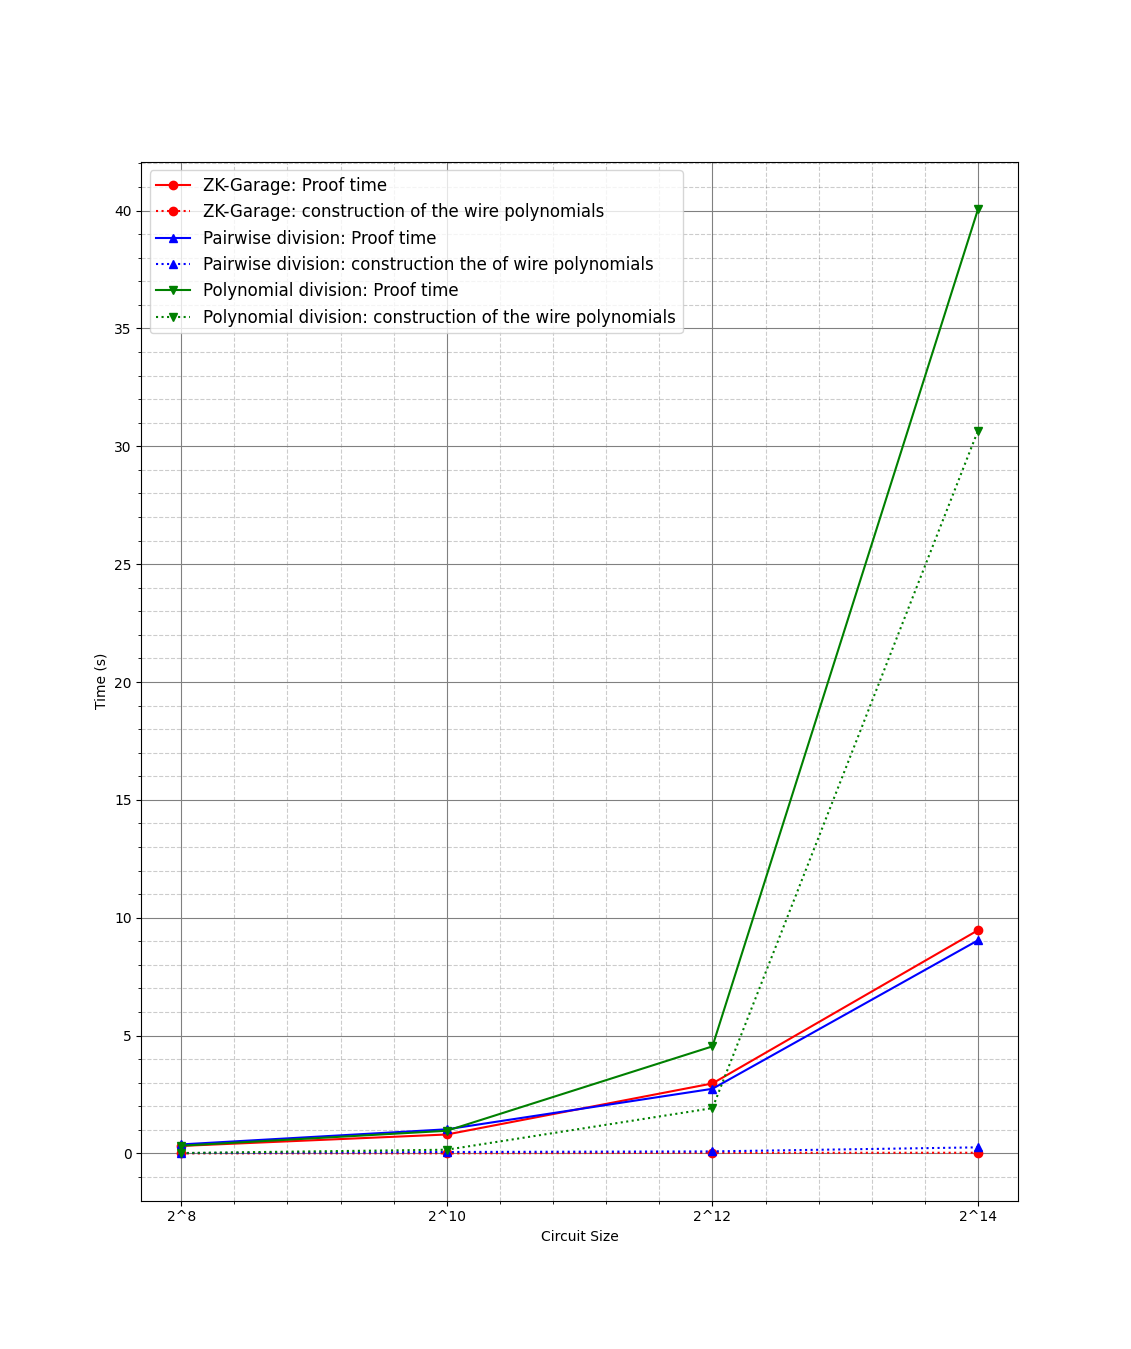
\includegraphics[width=1\linewidth]{figures/optimizations/local_bench.png}
    \caption{Local benchmarks on AMD Ryzen 7 5800H}
    \label{fig:local-bench}
\end{figure}

I compared the two implementations from \Cref{poly-div} and \Cref{pairwise-div} against the reference implementation. At first, I ran the benchmarks locally on a consumer-grade notebook. The major limitation was the memory capacity due to the size of SRS. I measured the total proving time and the time needed to construct the wire polynomials. The plot in \Cref{fig:local-bench} shows that the version with a naive polynomial division is unsurprisingly much worse than the ZK-Garage implementation. Construction of the wire polynomials alone takes 3 times the construction of the proof in ZK-Garage. Therefore, I will not consider this approach in further benchmarks. 

The alternative with pairwise division \Cref{pairwise-div} introduces overhead in the construction of the wire polynomials because it introduces additional $\fft$s. The improvement raises with the size of the circuit, which follows from the fact that the increased size of the circuit leads to greater padding. And the bigger the padding is, the more we can reduce the degree of the wire polynomials, resulting in improvements in rounds 2-5. So, for circuits of bigger size, the performance benefit becomes more pronounced. However, the improvement is much lower than what we were hoping for. To get insight into the problem, I measured what was happening in rounds 2-5. 

\subsection{Remote benchmarks}
The rest of the measurements were taken on servers of the Department of Applied Mathematics of the Faculty of Mathematics and Physics of Charles University. The machine has CPU type \textit{Intel Xeon E5-2630 v3} with 16 cores and frequency 3200 MHz. The memory usage after the setup of the protocol for the circuit of size $2^{20}$ reached 50GB, and the whole protocol filled the entire memory of 125GB on the circuit of size $2^{21}$. In addition to the proving time and the construction of wire polynomial $a(x), b(x), c(x)$, I have measured also commitments to these polynomials $[a]_1, [b]_1, [c]_1$ and also commitments to the quotient polynomial that is split into multiple parts as described in the round 3. Table \ref{table-measurements} shows the exact comparison between the reference implementation and the degree reduction described by pairwise division in the coset \ref{pairwise-div} in seconds. These results are as well plotted on \Cref{fig:kam-bench}.

\label{table-measurements}
\begin{table}[H]
    \centering
    \begin{tabular}{|l|llll|llll|}
    \hline
     &
      \multicolumn{4}{c|}{ZK-Garage} &
      \multicolumn{4}{c|}{Reduced Degree} \\ \hline
    \multicolumn{1}{|l|}{\begin{tabular}[c]{@{}l@{}}Circuit\\ size\end{tabular}} & 
      \multicolumn{1}{l|}{\begin{tabular}[c]{@{}l@{}}$a(x)$\\ $b(x)$\\ $c(x)$\end{tabular}} &
      \multicolumn{1}{l|}{\begin{tabular}[c]{@{}l@{}}$[a]_1$\\ $[b]_1$\\ $[c]_1$\end{tabular}} &
      \multicolumn{1}{l|}{$[t]_1$} &
    \multicolumn{1}{l|}{\begin{tabular}[c]{@{}l@{}}Proof\\ time\end{tabular}} & 
      \multicolumn{1}{l|}{\begin{tabular}[c]{@{}l@{}}$a(x)$\\ $b(x)$\\ $c(x)$\end{tabular}} &
      \multicolumn{1}{l|}{\begin{tabular}[c]{@{}l@{}}$[a]_1$\\ $[b]_1$\\ $[c]_1$\end{tabular}} &
      \multicolumn{1}{l|}{$[t]_1$} &
   \multicolumn{1}{l|}{\begin{tabular}[c]{@{}l@{}}Proof\\ time\end{tabular}} \\ \hline
    $2^{15}$ &
      \multicolumn{1}{l|}{0.023} &
      \multicolumn{1}{l|}{0.413} &
      \multicolumn{1}{l|}{0.466} &
      7.393 &
      \multicolumn{1}{l|}{0.102} &
      \multicolumn{1}{l|}{0.260} &
      \multicolumn{1}{l|}{0.467} &
      7.000 \\ \hline
    $2^{16}$ &
      \multicolumn{1}{l|}{0.039} &
      \multicolumn{1}{l|}{0.834} &
      \multicolumn{1}{l|}{0.856} &
      14.325 &
      \multicolumn{1}{l|}{0.183} &
      \multicolumn{1}{l|}{0.491} &
      \multicolumn{1}{l|}{0.883} &
      13.882 \\ \hline
    $2^{17}$ &
      \multicolumn{1}{l|}{0.061} &
      \multicolumn{1}{l|}{1.499} &
      \multicolumn{1}{l|}{1.487} &
      27.369 &
      \multicolumn{1}{l|}{0.341} &
      \multicolumn{1}{l|}{0.843} &
      \multicolumn{1}{l|}{1.489} &
      26.035 \\ \hline
    $2^{18}$ &
      \multicolumn{1}{l|}{0.133} &
      \multicolumn{1}{l|}{2.894} &
      \multicolumn{1}{l|}{2.954} &
      54.144 &
      \multicolumn{1}{l|}{0.692} &
      \multicolumn{1}{l|}{1.642} &
      \multicolumn{1}{l|}{2.972} &
      52.479 \\ \hline
    $2^{19}$ &
      \multicolumn{1}{l|}{0.244} &
      \multicolumn{1}{l|}{5.393} &
      \multicolumn{1}{l|}{5.110} &
      106.628 &
      \multicolumn{1}{l|}{1.268} &
      \multicolumn{1}{l|}{3.182} &
      \multicolumn{1}{l|}{5.310} &
      103.123 \\ \hline
    $2^{20}$ &
      \multicolumn{1}{l|}{0.499} &
      \multicolumn{1}{l|}{9.166} &
      \multicolumn{1}{l|}{9.166} &
      201.599 &
      \multicolumn{1}{l|}{2.615} &
      \multicolumn{1}{l|}{5.555} &
      \multicolumn{1}{l|}{10.817} &
      198.667 \\ \hline
    \end{tabular}
\end{table}

\begin{figure}
    \centering
    \label{fig:kam-bench}
    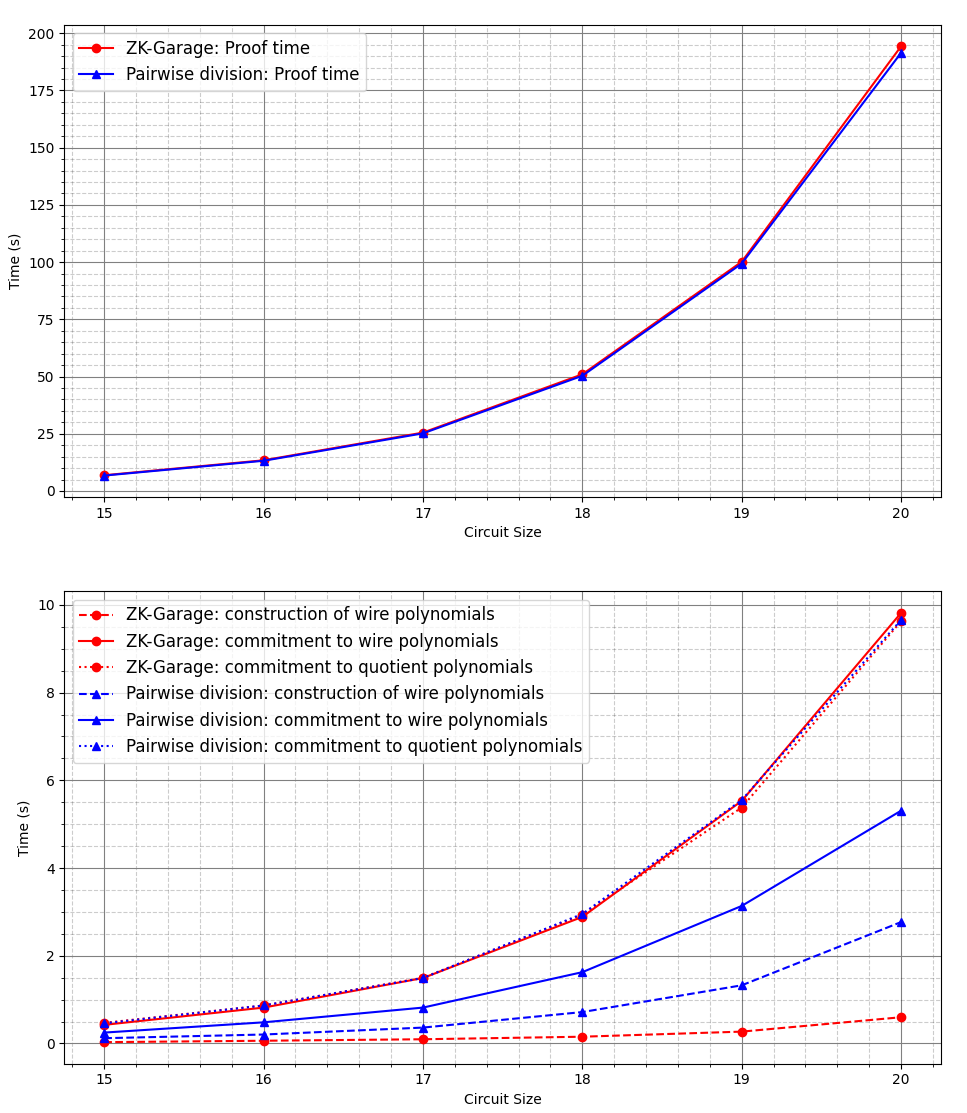
\includegraphics[width=1\linewidth]{figures/optimizations/kam_bench.png}
    \caption{Remote benchmarks on Intel Xeon E5-2630 v3}
\end{figure}

It is again evident that the improvement in the proof time is negligible. Time for the commitment of the wire polynomial decreased significantly as it should; however, the commitment of the quotient polynomial did not change at all. In this optimization, we wanted to reduce the degree of the wire polynomial with the hope the polynomial $t(x)$ constructed from the wire polynomials would also have a smaller degree. Since commitments to the quotient polynomial take approximately the same time and the complexity of commitment is dominated MSM, it must mean that the degree of the quotient polynomial $t(x)$ does not change at all. 

Going back to the ZK-Garage implementation, I found out that the quotient polynomial is computed in the evaluation form, unlike the protocol description in the original paper \cite{plonk}. First, all of the required polynomials are transformed into a coset of the domain $H$ of size 8n. This is due to a similar reason as in \Cref{pairwise-div} to avoid division by 0. Each of the parts of the quotient polynomial is computed in the evaluation form. Finally, they are merged and interpolated through coset-$\ifft$. The resulting polynomial is split into 8 parts, and the prover calculates the commitment to each of them. The reason why the polynomial needs to be split into 8 parts is that the \Cref{eq:gate-contraints} is extended with checks for custom gates, and there is also an additional polynomial proving the validity of the lookup table. As a result, the degree of $t(x)$ is determined by interpolation, and the reduction of the wire polynomial does not affect the degree of the quotient polynomial. 

\begin{pchstack}[center, boxed]
    \pseudocode[linenumbering, head=ZK-Garage Round 3] {
        \text{evaluate polynomial on coset of domain of size } 8n \\
        \text{calculate } t_1(x) \ref{quotient1}, t_2(x) \ref{quotient2} t_3(x) \ref{quotient3} \text{ in the evaluation form} \\
        \text{calculate polynomial } t_4(x) \text{ for proving correctness of the lookup table } \\
        \text{merge and interpolate } t(x) = \cifft(t_1(x) + t_2(x) + t_3(x) + t_4(x)) \\ 
        \text{split the result into 8 polynomials and calculate corresponding commitments }
    }
\end{pchstack}

We can conclude that the only performance benefit of the optimization \ref{pairwise-div} is in the computation of commitments $[a]_1, [b]_1, [c]_1$ and the quotient polynomial is computed from evaluations of wire polynomials. We know that it is possible to compute the commitment form a polynomial in evaluation form as explained in \Cref{sec:kzg-evaluation-form}, so if it even needed to construct the polynomials $a(x), b(x), c(x)$? Round 3 uses the evaluation wire polynomials in the cost of the domain, which is easy to compute. The problem is that there are $8n$ evaluations instead of $n$. We have described how to compute a new evaluation with precomputed barycentric weights in $n$ operation. That means calculating the evaluations on the domain of size 8n will take $8n^2$, which is slow. However, if there is a smarter way to do this that is comparable to $n \log{n}$, we could skip the computation of $ a(x), b(x), c(x)$ together. 

In conclusion, the optimization with degree reduction of the wire polynomials did not bring the desired performance benefit for this implementation of the $\plonk$ protocol due to the reason that round 3 is computed in another way than in the description of the protocol. 

\subsection{Engineering approach}
Designing a more efficient variant of the $\plonk$ protocol is undoubtedly a hard task, and sometimes, an engineering approach might produce good results. Even though this was not the purpose of the work, there are many possible improvements on the software side. The most notable difference was produced by parallelized computations in round 2 and round 3. As already discussed, the construction of the wire protocol takes a significant portion of the proving time, which becomes even more pronounced for circuits of larger size. Since the quotient polynomial is computed in the evaluation form, the whole computation is trivially parallelizable. We improved the function for computing $t(x)$ by a parallelized approach to computing the evaluation of the polynomial for gate constraints, permutation constraints, and lookup table constraints. A similar approach also helped to speed up the construction of the permutation polynomial $z(x)$ in round 2. This approach was implemented using the parallel iterator in \href{https://github.com/rayon-rs/rayon}{rayon}, which is a lightweight data parallelism library that guarantees data race freedom. In the next measurement, we compared the approach \Cref{pairwise-div} with parallel computation of $t(x)$ and $z(x)$. As can be seen from the results \Cref{fig:parallelized}, this change yields a significantly faster prover algorithm. 

\begin{table}[H]
\scriptsize
\begin{tabular}{|l|lll|lll|lll|}
\hline
 &
  \multicolumn{3}{c|}{permutaiton polynomial} &
  \multicolumn{3}{c|}{quotient polynomial} &
  \multicolumn{3}{c|}{total proof time} \\ \hline
Degree &
  \multicolumn{1}{l|}{zkg.} &
  \multicolumn{1}{l|}{par.} &
  imp. &
  \multicolumn{1}{l|}{zkg.} &
  \multicolumn{1}{l|}{par.} &
  imp. &
  \multicolumn{1}{l|}{zkg.} &
  \multicolumn{1}{l|}{par.} &
  imp. \\ \hline
$2^{15}$ &
  \multicolumn{1}{l|}{0.23} &
  \multicolumn{1}{l|}{0.05} &
  76.52\% &
  \multicolumn{1}{l|}{3.72} &
  \multicolumn{1}{l|}{1.41} &
  62.13\% &
  \multicolumn{1}{l|}{6.84} &
  \multicolumn{1}{l|}{4.18} &
  38.88\% \\ \hline
$2^{16}$ &
  \multicolumn{1}{l|}{0.46} &
  \multicolumn{1}{l|}{0.10} &
  77.73\% &
  \multicolumn{1}{l|}{7.40} &
  \multicolumn{1}{l|}{2.77} &
  62.58\% &
  \multicolumn{1}{l|}{13.39} &
  \multicolumn{1}{l|}{8.13} &
  39.28\% \\ \hline
$2^{17}$ &
  \multicolumn{1}{l|}{0.89} &
  \multicolumn{1}{l|}{0.18} &
  79.42\% &
  \multicolumn{1}{l|}{14.72} &
  \multicolumn{1}{l|}{5.56} &
  62.25\% &
  \multicolumn{1}{l|}{25.55} &
  \multicolumn{1}{l|}{15.16} &
  40.66\% \\ \hline
$2^{18}$ &
  \multicolumn{1}{l|}{1.80} &
  \multicolumn{1}{l|}{0.33} &
  81.58\% &
  \multicolumn{1}{l|}{29.56} &
  \multicolumn{1}{l|}{11.64} &
  60.63\% &
  \multicolumn{1}{l|}{51.02} &
  \multicolumn{1}{l|}{30.48} &
  40.26\% \\ \hline
$2^{19}$ &
  \multicolumn{1}{l|}{3.55} &
  \multicolumn{1}{l|}{0.66} &
  81.44\% &
  \multicolumn{1}{l|}{59.56} &
  \multicolumn{1}{l|}{23.24} &
  60.99\% &
  \multicolumn{1}{l|}{100.75} &
  \multicolumn{1}{l|}{59.26} &
  41.18\% \\ \hline
$2^{20}$ &
  \multicolumn{1}{l|}{7.11} &
  \multicolumn{1}{l|}{1.37} &
  80.71\% &
  \multicolumn{1}{l|}{120.17} &
  \multicolumn{1}{l|}{47.00} &
  60.89\% &
  \multicolumn{1}{l|}{195.09} &
  \multicolumn{1}{l|}{112.38} &
  42.40\% \\ \hline
\end{tabular}
\end{table}

While we have mentioned other design optimizations of the protocol, it might be also meaningful to work on an engineering solution. There have already been multiple attempts for hardware optimization of computationally expensive tasks like MSM, one of which is covered in the paper \cite{pipeMSM}.


\begin{figure}
    \centering
    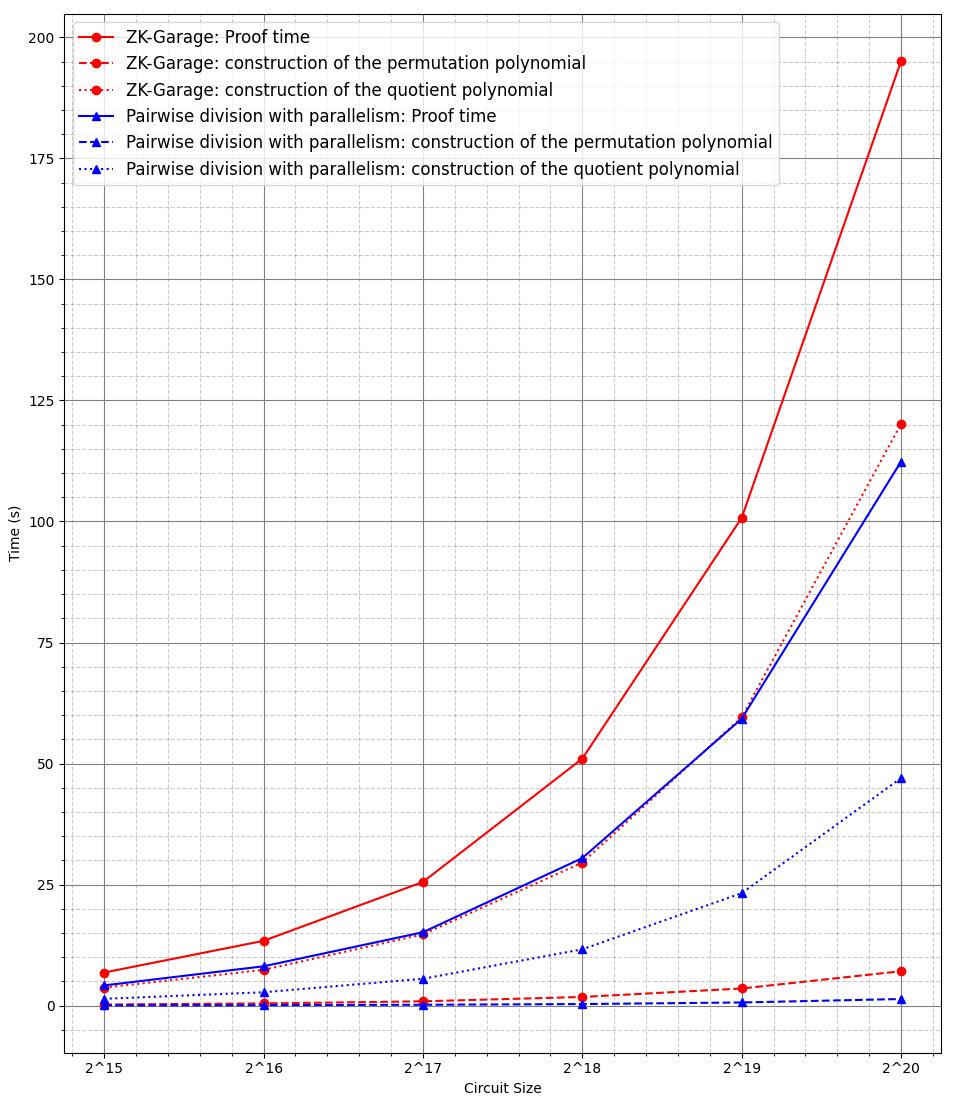
\includegraphics[width=1\linewidth]{figures//optimizations/parallel.png}
    \caption{Parallel computation of the quotient polynomial}
    \label{fig:parallelized}
\end{figure}
